% This file was converted to LaTeX by Writer2LaTeX ver. 1.0.2
% see http://writer2latex.sourceforge.net for more info
\documentclass[twoside,letterpaper]{article}
\usepackage[latin1]{inputenc}
\usepackage[T1]{fontenc}
\usepackage[english]{babel}
\usepackage{amsmath}
\usepackage{amssymb,amsfonts,textcomp}
\usepackage{color}
\usepackage{array}
\usepackage{supertabular}
\usepackage{hhline}
\usepackage{hyperref}
\hypersetup{pdftex, colorlinks=true, linkcolor=blue, citecolor=blue, filecolor=blue, urlcolor=blue, pdftitle=SYSTEM AND SOFTWARE ARCHITECTURAL AND DETAILED DESIGN DESCRIPTI, pdfauthor=Clinton Jeffery, pdfsubject=, pdfkeywords=}
\usepackage[pdftex]{graphicx}
% Outline numbering
\setcounter{secnumdepth}{5}
\renewcommand\thesection{\arabic{section}}
\renewcommand\thesubsection{\arabic{section}.\arabic{subsection}}
\renewcommand\thesubsubsection{\arabic{section}.\arabic{subsection}.\arabic{subsubsection}}
\renewcommand\theparagraph{\arabic{section}.\arabic{subsection}.\arabic{subsubsection}.\arabic{paragraph}}
\renewcommand\thesubparagraph{\arabic{section}.\arabic{subsection}.\arabic{subsubsection}.\arabic{paragraph}.\arabic{subparagraph}}
\makeatletter
\newcommand\arraybslash{\let\\\@arraycr}
\makeatother
% List styles
\newcommand\liststyleWWviiiNumii{%
\renewcommand\theenumi{\arabic{enumi}}
\renewcommand\theenumii{\arabic{enumii}}
\renewcommand\theenumiii{\arabic{enumiii}}
\renewcommand\theenumiv{\arabic{enumiv}}
\renewcommand\labelenumi{\theenumi)}
\renewcommand\labelenumii{\theenumii.}
\renewcommand\labelenumiii{\theenumiii.}
\renewcommand\labelenumiv{\theenumiv.}
}
% Page layout (geometry)
\setlength\voffset{-1in}
\setlength\hoffset{-1in}
\setlength\topmargin{0.5in}
\setlength\oddsidemargin{1in}
\setlength\evensidemargin{1in}
\setlength\textheight{8.278in}
\setlength\textwidth{6.5in}
\setlength\footskip{0.561in}
\setlength\headheight{0.5in}
\setlength\headsep{0.461in}
% Footnote rule
\setlength{\skip\footins}{0.0469in}
\renewcommand\footnoterule{\vspace*{-0.0071in}\setlength\leftskip{0pt}\setlength\rightskip{0pt plus 1fil}\noindent\textcolor{black}{\rule{0.25\columnwidth}{0.0071in}}\vspace*{0.0398in}}
% Pages styles
\makeatletter
\newcommand\ps@Standard{
  \renewcommand\@oddhead{}
  \renewcommand\@evenhead{\@oddhead}
  \renewcommand\@oddfoot{\foreignlanguage{english}{\textcolor{black}{\hfill SSDD Page }}{\textcolor{black}{\thepage{}}}}
  \renewcommand\@evenfoot{\@oddfoot}
  \renewcommand\thepage{\arabic{page}}
}
\newcommand\ps@Convertix{
  \renewcommand\@oddhead{}
  \renewcommand\@evenhead{\@oddhead}
  \renewcommand\@oddfoot{}
  \renewcommand\@evenfoot{\@oddfoot}
  \renewcommand\thepage{\arabic{page}}
}
\newcommand\ps@Convertviii{
  \renewcommand\@oddhead{}
  \renewcommand\@evenhead{\@oddhead}
  \renewcommand\@oddfoot{}
  \renewcommand\@evenfoot{\@oddfoot}
  \renewcommand\thepage{\arabic{page}}
}
\newcommand\ps@Convertvii{
  \renewcommand\@oddhead{}
  \renewcommand\@evenhead{\@oddhead}
  \renewcommand\@oddfoot{}
  \renewcommand\@evenfoot{\@oddfoot}
  \renewcommand\thepage{\arabic{page}}
}
\newcommand\ps@Convertvi{
  \renewcommand\@oddhead{}
  \renewcommand\@evenhead{\@oddhead}
  \renewcommand\@oddfoot{}
  \renewcommand\@evenfoot{\@oddfoot}
  \renewcommand\thepage{\arabic{page}}
}
\newcommand\ps@Convertiv{
  \renewcommand\@oddhead{}
  \renewcommand\@evenhead{\@oddhead}
  \renewcommand\@oddfoot{}
  \renewcommand\@evenfoot{\@oddfoot}
  \renewcommand\thepage{\arabic{page}}
}
\newcommand\ps@FirstPage{
  \renewcommand\@oddhead{}
  \renewcommand\@evenhead{\@oddhead}
  \renewcommand\@oddfoot{\foreignlanguage{english}{\textcolor{black}{\hfill SSDD Page }}
{\textcolor{black}{\thepage{}}}}
  \renewcommand\@evenfoot{\@oddfoot}
  \renewcommand\thepage{\arabic{page}}
}
\makeatother
\pagestyle{Standard}
\setlength\tabcolsep{1mm}
\renewcommand\arraystretch{1.3}
\title{SYSTEM AND SOFTWARE ARCHITECTURAL AND DETAILED DESIGN DESCRIPTI}
\author{Clinton Jeffery}
\date{2010-11-18T11:30:10.24}
\begin{document}


\clearpage

{\centering\selectlanguage{english}\bfseries\color{black}
SYSTEM AND SOFTWARE DESIGN DESCRIPTION (SSDD): Incorporating
Architectural Views and Detailed Design Criteria
\par}

{\centering\selectlanguage{english}\bfseries\color{black}
FOR
\par}


\bigskip

{\centering\selectlanguage{english}\bfseries\color{black}
Phunctional UML Editor
\\(pUML)
\par}


\bigskip


\bigskip


\bigskip

{\centering \par}

\begin{figure}
\centering

\includegraphics[width=3.4354in,height=0.6126in]{SSDDTemplateA2-img1.png}
\end{figure}

\bigskip


\bigskip


\bigskip


\bigskip

{\centering\selectlanguage{english}\bfseries\color{black}
Version 0.0
\par}

{\centering\selectlanguage{english}\bfseries\color{black}
January 30, 2012
\par}


\bigskip


\bigskip

{\centering\selectlanguage{english}\bfseries\color{black}
Prepared for:
\par}
{\centering\selectlanguage{english}\bfseries\color{black}
Bruce Bolden
\par}
{\centering\selectlanguage{english}\bfseries\color{black}
and
\par}
{\centering\selectlanguage{english}\bfseries\color{black}
Dr. Clint Jeffery
\par}

\bigskip


\bigskip

{\centering\selectlanguage{english}\bfseries\color{black}
Prepared by:
\par}

{\centering\selectlanguage{english}\bfseries\color{black}
Josh Armstrong
\\Zach Curtis
\\Brian Bowles
\\Logan Evans
\\Jeremy Klas
\\Nathan Krussel
\\Maxine Major
\\Morgan Weir
\\David Wells
\\and
\\Xiaozhe Shen
\par}

{\centering\selectlanguage{english}\bfseries\color{black}
University of Idaho
\par}

{\centering\selectlanguage{english}\bfseries\color{black}
Moscow, ID \ 83844-1010
\par}

\clearpage{\centering\selectlanguage{english}\bfseries\color{black}
CS383 SSDD
\par}










{\centering\selectlanguage{english}\bfseries\color{black}
RECORD OF CHANGES (Change History)
\par}

\begin{flushleft}
\tablehead{}
\begin{supertabular}{|m{1.0in}|m{0.6in}|p{1.5in}|m{.25in}|m{2.0in}|m{.7in}|m{0.65in}|}
\hline
~

\centering {\selectlanguage{english}\bfseries\color{black} Change}\par

\centering {\selectlanguage{english}\bfseries\color{black} Number}\par

~
 &
~

\centering \selectlanguage{english}\bfseries\color{black} Date completed
&
~

\centering {\selectlanguage{english}\bfseries\color{black} Location of
change }\par

\centering \selectlanguage{english}\bfseries\color{black} (e.g., page or
figure \#) &
~

\centering {\selectlanguage{english}\bfseries\color{black} A}\par

\centering \selectlanguage{english}\bfseries\color{black} M\newline
D  &
~

\centering {\selectlanguage{english}\bfseries\color{black} Brief
description }\par

\centering \selectlanguage{english}\bfseries\color{black} of change &
~

\centering \selectlanguage{english}\bfseries\color{black} Approved by
(initials) &
~

\centering {\selectlanguage{english}\bfseries\color{black} Date }\par

\centering\arraybslash \selectlanguage{english}\bfseries\color{black}
approved\\\hline
~
 df84c744c60f &
~
 11/02/11 &
~
 hg/code/QT Project &
~
 A &
~
Added code stubs for node implementation (nodes.cpp, diagrams.cpp, etc) &
~
LE &
~
 11/02/11

\\\hline
~
 eae63bed20d2 &
~
 11/2/11 &
~
 /.hgignore &
~
 A &
~
 added .hgignore &
~
LE &
~
11/2/11

\\\hline
~
b119831d6fea &
~
11/6/11 &
~
N/A &
~
M &
~
organized submitted material into folders &
~
LE &
~
11/6/11

\\\hline
~
82fe1ebeeade &
~
11/6/11 &
~
/.hgignore &
~
M &
~
.hgignore to ignore file locks. &
~
LE &
~
11/6/11

\\\hline
~
6bf8d2e6f033 &
~
11/6/11 &
~
/hg/documentation/ html &
~
A &
~
Added the html doxygen output to the repository &
~
Auto &
~
11/6/11


\\\hline
~
db54296b4deb &
~
11/11/11 &
~
hg/documentation/ UMLsymbols &
~
A &
~
Updated folder with UML Symbols documentation &
~
MM &
~
11/11/11


\\\hline
~
1cca683da3f3 &
~
11/13/11 &
~
/hg/code/mainwindow/ &
~
A &
~
Added makefile &
~
LE &
~
11/13/11


\\\hline
~
4d98e0c6a896 &
~
11/13/11 &
~
hg/code/mainwindow/ &
~
A &
~
submitted UML menu (mainwindow.cpp, GUI.h, etc) &
~
XS &
~
11/13/11


\\\hline
~
efce0b2f8a24 &
~
11/13/11 &
~
hg/code/ &
~
A &
~
added pUML.cpp &
~
LE &
~
11/13/11


\\\hline
~
2f45b5a240af &
~
11/17/11 &
~
hg/code/Doagram Objects/ &
~
A &
~
QT drawing funcitons of circle and actor(circle.cpp...etc) &
~
ZC &
~
11/17/11


\\\hline
~
8f708577a183 &
~
12/2/11 &
~
hg/documentation/ &
~
A &
~
added UML diagrams and screen shots (use case, interaction, etc) &
~
MM &
~
12/2/2011


\\\hline
~
ec72fce5eb27 &
~
12/4/11 &
~
hg/code/mainwindow/ &
~
A &
~
Dialog for file->New &
~
DW &
~
12/4/11

\\\hline
~
442733ec36c2 &
~
12/4/11 &
~
hg/code/mainwindow/  &
~
M &
~
Modified Shen's mainwindow code to gray out tool bars. &
~
DW &
~
12/4/11


\\\hline
~
8712d7dd4c91 &
~
12/4/11 &
~
hg/code/mainwindow/ makefile &
~
D &
~
fixed case collision with Makefile and makefile &
~
JA &
~
12/4/11


\\\hline
~
cc9ebc151eb9 &
~
12/5/11 &
~
hg/code/mainwindow/ &
~
A &
~
Created canvas to allow for drawing area within the main window &
~
JA &
~
12/5/11



\\\hline
~
6d8c31be300e &
~
12/6/11 &
~
/hg/Presentation &
~
A &
~
Submitted User Manual/power point presentation &
~
MM &
~
12/6/11


\\\hline
~
93098598b83f &
~
12/8/11 &
~
hg/documentation/dox &
~
A &
~
created script to run doxygen on all folders inside puml/code &
~
LE &
~
12/8/11

\\\hline
~
 &
~
 &
~
 &
~
 &
~
 &
~
 &
~
\\\hline
~
 &
~
 &
~
 &
~
 &
~
 &
~
 &
~
\\\hline
~
 &
~
 &
~
 &
~
 &
~
 &
~
 &
~
\\\hline
~
 &
~
 &
~
 &
~
 &
~
 &
~
 &
~
\\\hline
~
 &
~
 &
~
 &
~
 &
~
 &
~
 &
~
\\\hline
\end{supertabular}
\end{flushleft}
{\selectlanguage{english}\color{black}
A - ADDED \ M - MODIFIED \ D -- DELETED}

\clearpage{\centering\selectlanguage{english}\bfseries\color{black}
Phunctional UML Editor
\par}

{\centering\selectlanguage{english}\bfseries\color{black}
TABLE OF CONTENTS
\par}

{\selectlanguage{english}\bfseries\color{black}
Section\ \ Page}

\setcounter{tocdepth}{9}
\renewcommand\contentsname{}
\tableofcontents

\bigskip

\bigskip
\clearpage\setcounter{page}{1}\pagestyle{Convertiv}
\section[INTRODUCTION]{\selectlanguage{english}\bfseries\color{black}
INTRODUCTION}

\subsection{IDENTIFICATION}

{\selectlanguage{english}\color{black}
This document has no identification numbers or applicable
revisions at this time.  All references in this document,
excepting items detailed in the change log, may be referenced
as revision 0 at this time.

\subsection[DOCUMENT PURPOSE, SCOPE, AND INTENDED
AUDIENCE]{\selectlanguage{english}\bfseries\color{black} DOCUMENT
PURPOSE, SCOPE, AND INTENDED AUDIENCE}

\subsubsection{Document Purpose}
{\selectlanguage{english}\color{black}
Phunctional UML Editor software was designed as a graded project for
Software Engineering, under the oversight and guidance of Professor
Bruce Bolden, at the Unversity of Idaho.  This document is required
as part of the graded assignment, and provides minimal insight to the
design of this incomplete project.  
}

\subsubsection{Document Scope and/or Context}
{\selectlanguage{english}\color{black}
This document includes information regarding the design and components of the pUML software.
}

\subsubsection{Intended Audience for Document}
{\selectlanguage{english}\color{black}
This document may be referenced for educational purposes by
Computer Science students and faculty at the University of Idaho.

}

\subsection[SYSTEM AND SOFTWARE PURPOSE, SCOPE, AND INTENDED
USERS]{\selectlanguage{english}\bfseries\color{black} SYSTEM AND
SOFTWARE PURPOSE, SCOPE, AND INTENDED USERS}


\subsubsection{System and Software Purpose}
{\selectlanguage{english}\color{black}
The pUML software is intended to be a tool utilized by software designers to create UML diagrams.
}

\subsubsection[System and Software Scope/or Context]{System and Software
Scope/or Context}
{\selectlanguage{english}\color{black}
The pUML software will be designed to provide functionality to create UML diagram projects.  Users will be able to create several different types of UML diagrams, create, modify, link, save, and delete objects within individual UML diagrams, and save collections of diagrams stored as part of a project.
}

\subsubsection{Intended Users for the System and Software}
{\selectlanguage{english}\color{black}
The completed product would be available to the general public for purchase.
}


\clearpage
\subsection[DEFINITIONS, ACRONYMS, AND
ABBREVIATIONS]{\selectlanguage{english}\bfseries\color{black}
DEFINITIONS, ACRONYMS, AND ABBREVIATIONS}
{\selectlanguage{english}\itshape\color{black}
This section shall list and define all special terms, acronyms and
abbreviations used throughout this document.}


\begin{flushleft}
\tablehead{\hline
\centering \selectlanguage{english}\bfseries\color{black} Term or
Acronym &
\centering\arraybslash \selectlanguage{english}\bfseries\color{black}
Definition\\\hline}
\begin{supertabular}{|m{1.3587599in}|m{5.00806in}|}
\selectlanguage{english}\color{black} Acquirer &
\selectlanguage{english}\color{black} The person, team, or organization
that pursues a system or software product or service from a supplier.
The acquirer may be a buyer, customer, owner, purchaser, or user.
\ ISO/IEC 42010:2007 (\S3.1).\\\hline
\selectlanguage{english}\color{black} AD &
\selectlanguage{english}\color{black} Architectural Description:
{\textquotedblleft}A collection of products to document an
architecture{\textquotedblright} ISO/IEC 42010:2007 (\S3.4).\\\hline
\selectlanguage{english}\color{black} Alpha test &
\selectlanguage{english}\color{black} Limited release(s) to selected,
outside testers\\\hline
\selectlanguage{english}\color{black} Architect &
\selectlanguage{english}\color{black}
\foreignlanguage{english}{{\textquotedblleft}}\foreignlanguage{english}{The
person, team, or organization responsible for systems
architecture{\textquotedblright} ISO/IEC 42010:2007 (\S3.2).}\\\hline
\selectlanguage{english}\color{black} Architectural Description &
\selectlanguage{english}\color{black} (AD) {\textquotedblleft}A
collection of products to document an architecture{\textquotedblright}
ISO/IEC 42010:2007 (\S3.4).\\\hline
\selectlanguage{english}\color{black} Architectural View &
\selectlanguage{english}\color{black}
\foreignlanguage{english}{{\textquotedblleft}}\foreignlanguage{english}{A
representation of a whole system from the perspective of a related set
of concerns{\textquotedblright} ISO/IEC 42010:2007 (\S3.9).}\\\hline
\selectlanguage{english}\color{black} Architecture &
\selectlanguage{english}\color{black}
\foreignlanguage{english}{{\textquotedblleft}}\foreignlanguage{english}{The
fundamental organization of a system embodied in its components, their
relationships to each other, and to the environment, and the principles
guiding its design and evolution{\textquotedblright} ISO/IEC 42010:2007
(\S3.5).}\\\hline
\selectlanguage{english}\color{black} Beta test &
\selectlanguage{english}\color{black} Limited release(s) to cooperating
customers wanting early access to developing systems\\\hline
\selectlanguage{english}\color{black} Design Entity &
\selectlanguage{english}\color{black}
\foreignlanguage{english}{{\textquotedblleft}}\foreignlanguage{english}{An
element (component) of a design that is structurally and functionally
distinct from other elements and that is separately named and
referenced{\textquotedblright} IEEE STD 1016-1998 (\S3.1).}\\\hline
\selectlanguage{english}\color{black} Design View &
\selectlanguage{english}\color{black}
\foreignlanguage{english}{{\textquotedblleft}}\foreignlanguage{english}{A
subset of design entity attribute information that is specifically
suited to the needs of a software project activity{\textquotedblright}
IEEE STD 1016-1998 (\S3.2).}\\\hline
\selectlanguage{english}\color{black} Final test &
\selectlanguage{english}\color{black} aka, Acceptance test, release of
full functionality to customer for approval\\\hline
\selectlanguage{english}\color{black} DFD &
\selectlanguage{english}\color{black} Data Flow Diagram\\\hline
\selectlanguage{english}\color{black} SDD &
\selectlanguage{english}\color{black} Software Design Document, aka SDS,
Software Design Specification\\\hline
\selectlanguage{english}\color{black} Software Design Description &
\selectlanguage{english}\color{black}
\foreignlanguage{english}{{\textquotedblleft}}\foreignlanguage{english}{A
representation of a software system created to facilitate analysis,
planning, implementation, and decision making, A blueprint or model of
a software system. The SDD is used as the primary medium for
communicating software }\foreignlanguage{english}{design
information{\textquotedblright} IEEE STD 1016-1998 (\S3.4).}\\\hline
\selectlanguage{english}\color{black} SRS &
\selectlanguage{english}\color{black} Software Requirements
Specification\\\hline
\selectlanguage{english}\color{black} SSDD &
\selectlanguage{english}\color{black} System and Software Design
Document\\\hline
\selectlanguage{english}\color{black} SSRS &
\selectlanguage{english}\color{black} System and Software Requirements
Specification\\\hline
\selectlanguage{english}\color{black} System &
\selectlanguage{english}\color{black}
\foreignlanguage{english}{{\textquotedblleft}}\foreignlanguage{english}{A
collection of components organized to accomplish a specific function or
set of functions{\textquotedblright} ISO/IEC 42010:2007
(\S3.7).}\\\hline
\selectlanguage{english}\color{black} System and Software Architecture
and Design Description &
\selectlanguage{english}\color{black} An architectural and detailed
design description that includes a software system within the context
of its enclosing system and describes the enclosing system, the
enclosed software, and their relationship and interfaces.\\\hline
\selectlanguage{english}\color{black} System Stakeholder &
\selectlanguage{english}\color{black}
\foreignlanguage{english}{{\textquotedblleft}}\foreignlanguage{english}{An
individual, team, or organization (or classes thereof) with interests
in, or concerns, relative to, a system{\textquotedblright} ISO/IEC
42010:2007 (\S3.8).}\\\hline
\end{supertabular}
\end{flushleft}
\subsection[DOCUMENT REFERENCES]{\selectlanguage{english}\bfseries\color{black} DOCUMENT
REFERENCES}

\liststyleWWviiiNumii
\begin{enumerate}
\item {\selectlanguage{english}\color{black}
\foreignlanguage{english}{CSDS,
}\foreignlanguage{english}{\textit{System and Software Requirements
Specification Template}}\foreignlanguage{english}{, Version 1.0, July
31, 2008, Center for Secure and Dependable Systems, University of
Idaho, Moscow, ID, 83844.}}
\item {\selectlanguage{english}\color{black}
\foreignlanguage{english}{ISO/IEC/IEEE,
}\foreignlanguage{english}{\textit{IEEE Std 1471-2000 Systems and
software engineering -- Recommended practice for architectural
description of software intensive systems,}}\foreignlanguage{english}{
First edition 2007-07-15, \ International Organization for
Standardization and International Electrotechnical Commission,
(ISO/IEC), Case postale 56, CH-1211 Gen\`{e}ve 20, Switzerland, and The
Institute of Electrical and Electronics Engineers, Inc., (IEEE), 445
Hoes Lane, Piscataway, NJ 08854, USA.}}
\item {\selectlanguage{english}\color{black}
\foreignlanguage{english}{IEEE, }\foreignlanguage{english}{\textit{IEEE
Std 1016-1998 Recommended Practice for Software Design
Descriptions}}\foreignlanguage{english}{, 1998-09-23, The Institute of
Electrical and Electronics Engineers, Inc., (IEEE) 445 Hoes Lane,
Piscataway, NJ 08854, USA.}}
\item {\selectlanguage{english}\color{black}
\foreignlanguage{english}{3) ISO/IEC/IEEE,
}\foreignlanguage{english}{\textit{IEEE Std. 15288-2008 Systems and
Software Engineering -- System life cycle
processes,}}\foreignlanguage{english}{ Second edition 2008-02-01,
\ International Organization for Standardization and International
Electrotechnical Commission, (ISO/IEC), Case postale 56, CH-1211 Gen\`{e}ve
20, Switzerland, and The Institute of Electrical and Electronics
Engineers, Inc., (IEEE), 445 Hoes Lane, Piscataway, NJ 08854, USA.}}
\item {\selectlanguage{english}\color{black}
\foreignlanguage{english}{ISO/IEC/IEEE, IEEE Std. 12207-2008,
}\foreignlanguage{english}{\textit{Systems and software engineering --
Software life cycle processes, }}\foreignlanguage{english}{Second
edition 2008-02-01, \ International Organization for Standardization
and International Electrotechnical Commission, (ISO/IEC), Case postale
56, CH-1211 }\foreignlanguage{english}{Gen\`{e}ve 20, Switzerland, and The
Institute of Electrical and Electronics Engineers, Inc., (IEEE), 445
Hoes Lane, Piscataway, NJ 08854, USA.}}
\end{enumerate}


\clearpage
\subsection{DOCUMENT OVERVIEW}

{\selectlanguage{english}\color{black}
Section 2 of this document describes the system and software constraints
imposed by the operational environment, system requirements and user
characteristics, and then identifies the system stakeholders and lists
describes their concerns and mitigations to those concerns.}

{\selectlanguage{english}\color{black}
Section 3 of this document describes the system and software
architecture from several viewpoints, including, but not limited to,
the developer{\textquoteright}s view and the user{\textquoteright}s
view.}

{\selectlanguage{english}\color{black}
Section 4 provides detailed design descriptions for every component
defined in the architectural view(s). \ Sections 5 provides
traceability information connecting the original specifications
(referenced above) to the architectural components and design entities
identified in this document.}

{\selectlanguage{english}\color{black}
Section 6 and beyond are appendices including original information and
communications used to create this document.}

\subsection[DOCUMENT
RESTRICTIONS]{\selectlanguage{english}\bfseries\color{black} DOCUMENT
RESTRICTIONS}

{\selectlanguage{english}\color{black}
This document is for LIMITED RELEASE ONLY to UI CS personnel working on
the project.}

\clearpage
\section{CONSTRAINTS AND STAKEHOLDER CONCERNS}

\subsection{CONSTRAINTS}

\subsubsection{Environmental Constraints.}
{\selectlanguage{english}\color{black}
The pUML software poses no environmental constraints at this time .
}

\subsubsection{System Requirement Constraints.}
{\selectlanguage{english}\color{black}
The pUML software will be designed to function on, at a minimum, Windows 7, Mac OSX, and Linux.  Cross platform functionality will minimize portability errors and allow for projects to be migrated between platforms with minimal difficulty.
}

\subsubsection{User Characteristic Constraints.}
{\selectlanguage{english}\color{black}
University of Idaho Computer Science students and faculty should be able
to reasonably understand and operate the pUML software.
}

\subsection[STAKEHOLDER CONCERNS]
{\selectlanguage{english}\bfseries\color{black} STAKEHOLDER CONCERNS}
{\selectlanguage{english}\color{black}
There are no stakeholders for our software at this time.
}


\bigskip





\clearpage\setcounter{page}{1}\pagestyle{Convertvi}
\section[SYSTEM AND SOFTWARE
ARCHITECTURE]{\selectlanguage{english}\bfseries\color{black} SYSTEM AND
SOFTWARE ARCHITECTURE}

\subsection[DEVELOPER{\textquoteright}S ARCHITECTURAL
VIEW]{\selectlanguage{english}\bfseries\color{black}
DEVELOPER{\textquoteright}S ARCHITECTURAL VIEW}

\subsubsection[Developer{\textquoteright}s View
Identification]{\selectlanguage{english}\bfseries\color{black}
Developer{\textquoteright}s View Identification}
{\selectlanguage{english}\color{black}
This is the architecture of the program from the viewpoint of the
developer. The purpose is to give an overview of the details of the major
components of the architecture.}

{\selectlanguage{english}\color{black}
In order to have the program be able to draw diagrams, a custom QWidget
is defined called the Canvas. The Canvas holds all the instatiations of
nodes and draws them all. It also creates the nodes by handling the
mouse click events. The toolbar and menu system lets the Canvas know
which type of object will be created next. The Canvas is a member of
the MainWindow class, which inherits from QMainWindow. }

\subsubsection[Developer{\textquoteright}s View Representation and
Description ]{Developer{\textquoteright}s View Representation and
Description }

{\selectlanguage{english}\color{black}
The Canvas contains a vector container of
ObjectNodes. Each ObjectNode has a draw function which takes a QPainter
reference as an argument and draws the appropriate figure with the
QPainter. The program then defines it's own ObjectNodes, e.g. CircleNode
and DiamondNode, and pushes them into the vector. In this way the Canvas
can draw each of the nodes in the diagram. To create a new object, it
handles a mouse click event and creates a new object of the type specified
by a previous call to it's function to set a new object type. The new
object is pushed into the vector and then the draw function is called
on every node in that vector. When selecting a node to edit or delete,
the Canvas takes the X and Y coordinates of the click and translates that
into the index of the object selected. Then the Canvas can popup a menu
to edit the node or delete the node. }


\subsubsection{Developer{\textquoteright}s Architectural Rationale}

{\selectlanguage{english}\color{black}
We decided to create a new QWidget for the Canvas so that it can handle
click events and have a paint function. We then decided to have the nodes
represented by a vector so that it can be easily iterated over and quickly
accessed by index. We decided to have the nodes be represented by specific
definitions of ObjectNodes so that they can all be pushed into the a vector
ObjectNodes. This way each of the nodes can define their own draw function,
as well private data such as radius for circles. This allows new objects to
be easily created. }

\clearpage
\subsection[USER{\textquoteright}S ARCHITECTURAL
VIEW]{\selectlanguage{english}\bfseries\color{black}
USER{\textquoteright}S ARCHITECTURAL VIEW}

\subsubsection{User{\textquoteright}s View Identification}

{\selectlanguage{english}\color{black}
This is the viewpoint of the program from the viewpoint of the user.
From this viewpoint, there are three major components of the
program: the Canvas, the Toolbar and the Menu. }

\subsubsection{User{\textquoteright}s View Representation and
Description }
{\selectlanguage{english}\color{black}
The menu and the toolbar have redundant functionality. The toolbar has
quick access to certain menu items. Either way, the user selects what object
he wants to draw and then clicks on the Canvas to draw them. Then the user
can select objects by clicking on them on the Canvas, and right clicking
on them to popup a menu. From the popup menu he can delete or edit the object.}

\subsection[CONSISTENCY OF ARCHITECTURAL
VIEWS]{\selectlanguage{english}\bfseries\color{black} CONSISTENCY OF
ARCHITECTURAL VIEWS}
{\selectlanguage{english}\color{black}
There are no known inconsistencies between views. }

\subsubsection{Detail of Inconsistencies between Architectural Views}
{\selectlanguage{english}\color{black}
NA}

\subsubsection{Consistency Analysis and Inconsistency Mitigations}
{\selectlanguage{english}\color{black}
NA}

\clearpage
\section{SOFTWARE DETAILED DESIGN}

\bigskip

\subsection[\ DEVELOPER{\textquoteright}S VIEWPOINT DETAILED SOFTWARE
DESIGN]{\foreignlanguage{english}{\ }\foreignlanguage{english}{DEVELOPER{\textquoteright}S
VIEWPOINT DETAILED SOFTWARE DESIGN}}

{\selectlanguage{english}\color{black}
The Canvas widget is the main viewpoint of our software design.  
All other classes either house this widget or support it.}

\subsection[COMPONENT/ENTITY DICTIONARY]{\selectlanguage{english}\bfseries\color{black} COMPONENT/ENTITY DICTIONARY}
{\selectlanguage{english}\color{black}
This table shows the individual components, implemented as classes, utilized in the development of this software,
and how each class is related to the other classes.}

\begin{flushleft}
\tablehead{}
\begin{supertabular}{|m{1.0462599in}|m{0.9837598in}|m{1.6712599in}|m{1.2962599in}|m{1.2580599in}|}
\hline
\multicolumn{5}{|m{6.57056in}|}{\centering
\selectlanguage{english}\bfseries\color{black} Component/Entity
Dictionary}\\\hline
\centering \selectlanguage{english}\bfseries\color{black} Name of Class &
\centering \selectlanguage{english}\bfseries\color{black} Type/Range &
\centering \selectlanguage{english}\bfseries\color{black}
Purpose/Function &
\centering \selectlanguage{english}\bfseries\color{black} Dependencies &
\centering\arraybslash \selectlanguage{english}\bfseries\color{black}
Subordinates
\\\hline
~ Main Window
&
~ QMainWindow
 &
~ To generate GUI and house Canvas
 &
~ N/A
 &
~ Canvas
\\\hline
~ Canvas
 &
~ QWidget
 &
~ To draw UML diagrams
 &
~ The Main Window
 &
~ N/A
\\\hline
~ Main Menu
 &
~ TBD
 &
~
 &
~
 &
~
\\\hline
~ QMenu
 &
~ TBD
 &
~
 &
~
 &
~
\\\hline
~ Toolbar
 &
~ TBD
 &
~
 &
~
 &
~
\\\hline
\end{supertabular}
\end{flushleft}

{\selectlanguage{english}\color{black}
Below is the diagram depicting classes and relationships between classes for the pUML software.}

\begin{figure}[h]
\centering
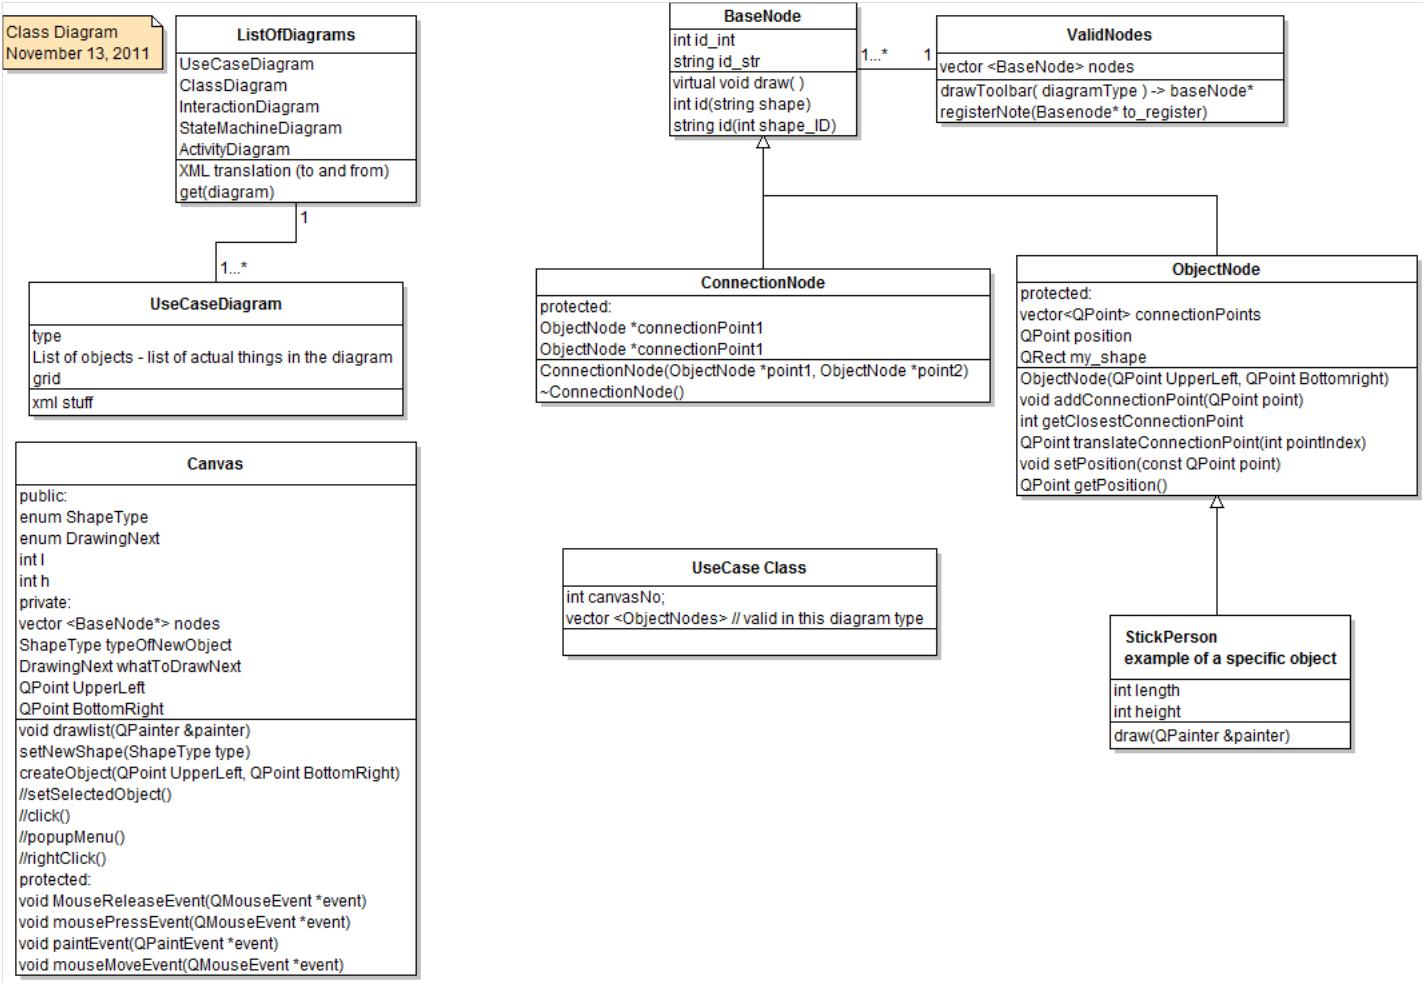
\includegraphics[width=6.0in]{class.jpg}
\end{figure}

\clearpage


\subsection[FEATURE DETAILED DESIGN]
{\selectlanguage{english}\bfseries\color{black} FEATURE DETAILED DESIGN}
{\selectlanguage{english}\color{black}
Each of the diagrams in this section represent an important functionality
of the pUML software.  The interaction diagrams detail the object classes
that will be utilized in the execution of each of these major features of
the software, as well as show how these classes interact.
}

\subsubsection{Detailed Design for Feature: Place New Object }

\paragraph[\ Introduction/Purpose of this Feature]
{\ Introduction/Purpose of this Feature}
{\selectlanguage{english}\color{black}
The user will be able to select objects from the toolbar and place them on the Canvas.
}

\paragraph[Input for this Feature]{Input for this Feature}
{\selectlanguage{english}\color{black}
The user will click on a shape on the toolbar.  The first subsequent click of the mouse over the Canvas area will place the selected shape at that location.
}

\paragraph{Output for this Feature}
{\selectlanguage{english}\color{black}
The object will be placed on the Canvas, at a location of the user{\textquoteright}s choosing, provided there are no collisions with other objects.
}

\paragraph{Feature Process to Convert Input to Output}
{\selectlanguage{english}\color{black}
The mouse click on a shape on the toolbar will lock that shape in memory.
The subsequent mouse click on the Canvas will send the shape information from the toolbar to the Canvas.  
The Canvas will draw the shape at the specific coordinates of the mouse click, and will update the list of existing shapes on the Canvas for that particular diagram.
}

\paragraph{Design Constraints and Performance Requirements of this Feature}
{\selectlanguage{english}\color{black}
The object will not be permitted to be placed at an overlapping location with another object.
}
\bigskip
\bigskip

\begin{figure}[h]
\centering
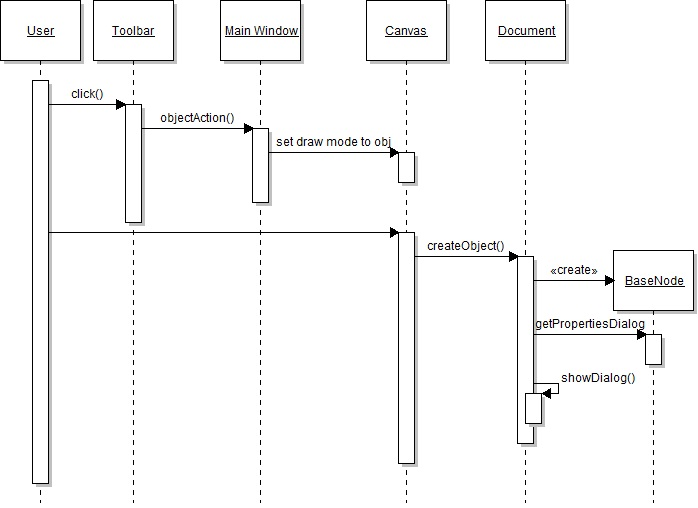
\includegraphics[width=6.0in]{IntNewObj.jpg}
\end{figure}

\clearpage


\subsubsection{Detailed Design for Feature: Place a New Connector}

\paragraph[\ Introduction/Purpose of this Feature]
{\ Introduction/Purpose of this Feature}
{\selectlanguage{english}\color{black}
This feature allows the user to place a connecting line between two objects.
}

\paragraph[Input for this Feature]{Input for this Feature}
{\selectlanguage{english}\color{black}
The user selects a connector shape from the toolbar, and then selects two objects between which to place the connector.
}

\paragraph{Output for this Feature}
{\selectlanguage{english}\color{black}
A connector line is drawn between the two objects the user selected.
}

\paragraph{Feature Process to Convert Input to Output}
{\selectlanguage{english}\color{black}
User clicks on a connector shape in the Toolbar.  
The Canvas gets the connector information from the Toolbar.  
The user clicks on an object.
The Canvas verifies that an object exists at that location, identifies the closest connection point on the object to the click, and stores this information.
The user clicks on a second object on the Canvas.  
The Canvas verifies that an object exists at the second location, identifies the closest connection point on the object to the click, and stores this information.  
The Canvas draws the connector at the coordinates of the user{\textquoteright}s click on the Canvas.  
Canvas updates list of objects on the Canvas.  
}

\paragraph{Design Constraints and Performance Requirements of this Feature}
{\selectlanguage{english}\color{black}
More than one connector may not connect the same two objects.
\\A connector may not be placed if two different objects have not been selected to place the connector between.
}
\bigskip
\bigskip

\begin{figure}[h]
\centering
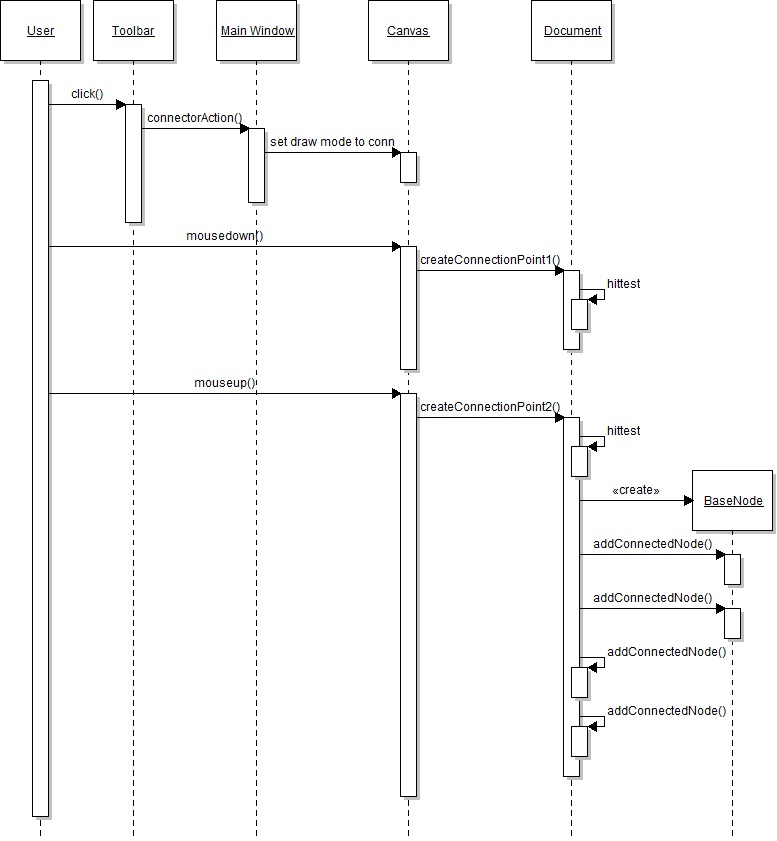
\includegraphics[width=5.0in]{IntNewConn.jpg}
\end{figure}

\clearpage

\subsubsection{Detailed Design for Feature: Edit an Object}

\paragraph[\ Introduction/Purpose of this Feature]
{\ Introduction/Purpose of this Feature}
{\selectlanguage{english}\color{black}
The user may edit an object{\textquoteright}s properties, such as names, descriptions, etc..
}

\paragraph[Input for this Feature]{Input for this Feature}
{\selectlanguage{english}\color{black}
The user right clicks on the object they wish to modify.
}

\paragraph{Output for this Feature}
{\selectlanguage{english}\color{black}
The program displays a dialog box with object properties the user may modify, and updates the program with changes.
}

\paragraph{Feature Process to Convert Input to Output}
{\selectlanguage{english}\color{black}
User right clicks on an object on the Canvas. The Canvas determines whether an object resides at those coordinates. If valid, the Canvas sets that object, and activates QMenu, which in turn shows the Dialog for the selected object.
The user modifies the object properties per the Dialog.  The Dialog sends the updated object information back to the Canvas.
}

\paragraph{Design Constraints and Performance Requirements of this Feature}
{\selectlanguage{english}\color{black}
The user may not edit Canvas properties.
}
\bigskip
\bigskip

\begin{figure}[h]
\centering
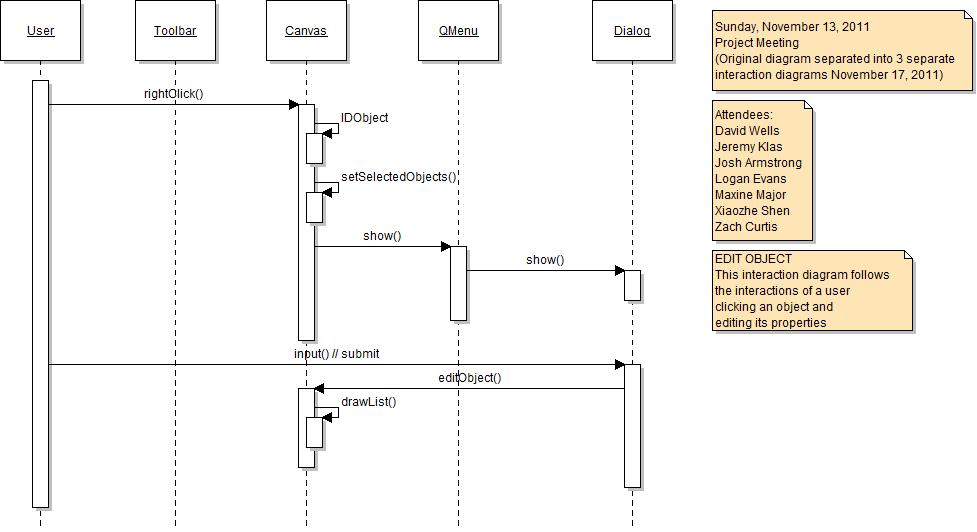
\includegraphics[width=6.0in]{IntEditObj.jpg}
\end{figure}

\clearpage


\subsubsection{Detailed Design for Feature: Edit a connector}

\paragraph[\ Introduction/Purpose of this Feature]
{\ Introduction/Purpose of this Feature}
{\selectlanguage{english}\color{black}
User may edit a connector{\textquoteright}s features, such as name, descriptors, arrowheads, direction, etc..
}

\paragraph[Input for this Feature]{Input for this Feature}
{\selectlanguage{english}\color{black}
The user right clicks on a connector.
}

\paragraph{Output for this Feature}
{\selectlanguage{english}\color{black}
A dialog is displayed from which the user may make changes to the connector{\textquoteright}s properties.
}

\paragraph{Feature Process to Convert Input to Output}
{\selectlanguage{english}\color{black}
User right clicks on a connector on the Canvas. The Canvas determines whether a connector resides at those coordinates. If valid, the Canvas sets that connector, and activates QMenu, which in turn shows the Dialog for the selected connector.
The user modifies the connector properties per the Dialog.  The Dialog sends the updated connector information back to the Canvas.
}

\paragraph{Design Constraints and Performance Requirements of this Feature}
{\selectlanguage{english}\color{black}
The user may not be able to edit all properties of all connectors due to the differences in connector utilization in differing UML diagrams.
}
\bigskip
\bigskip

\begin{figure}[h]
\centering
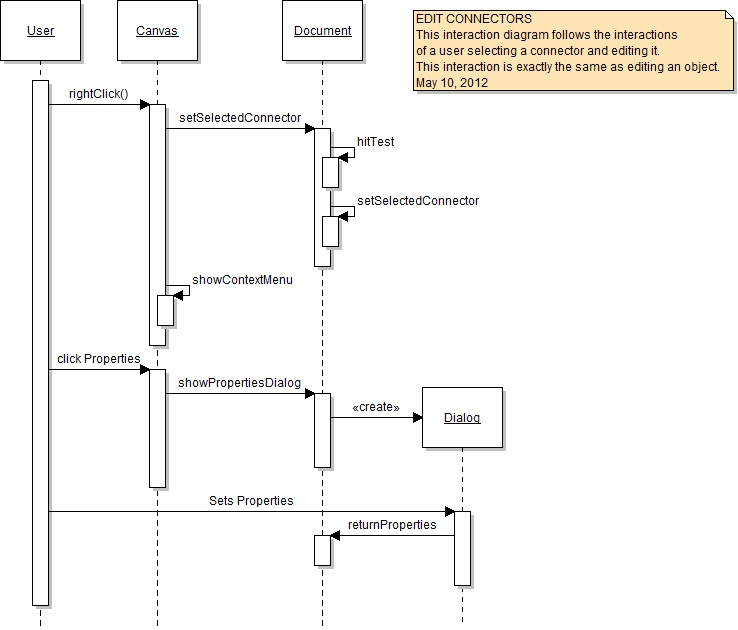
\includegraphics[width=6.0in]{IntEditConn.jpg}
\end{figure}

\clearpage

\subsubsection{Detailed Design for Feature: Select an Object}

\paragraph[\ Introduction/Purpose of this Feature]
{\ Introduction/Purpose of this Feature}
{\selectlanguage{english}\color{black}
User wishes to select an object, either for editing purposes or to move the object.
}

\paragraph[Input for this Feature]{Input for this Feature}
{\selectlanguage{english}\color{black}
User clicks on the object.
}

\paragraph{Output for this Feature}
{\selectlanguage{english}\color{black}
The canvas identifies and displays the object as selected.
}

\paragraph{Feature Process to Convert Input to Output}
{\selectlanguage{english}\color{black}
The user clicks on an object. Canvas stores the coordinates of the click and sends them to nodes to test whether an object resides at those coordinates on the Canvas.  nodes returns true or false. Canvas updates the index of selected items, and draws this list back to nodes.
}

\paragraph{Design Constraints and Performance Requirements of this Feature}
{\selectlanguage{english}\color{black}
Actions that may be based upon an object{\textquoteright}s selection have not been developed at this time.
}
\bigskip
\bigskip

\begin{figure}[h]
\centering
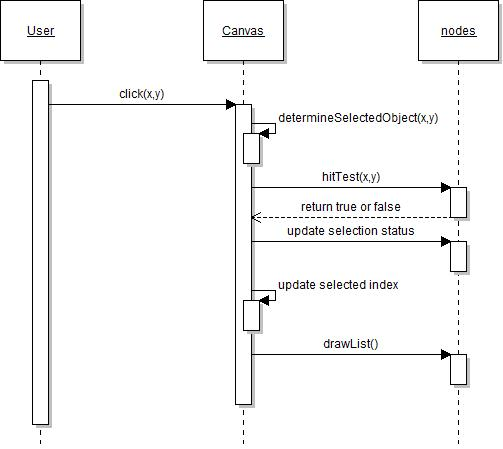
\includegraphics[width=5.0in]{IntSelectObj.jpg}
\end{figure}

\clearpage



 

\subsubsection{Detailed Design for Feature: Delete an Object}

\paragraph[\ Introduction/Purpose of this Feature]
{\ Introduction/Purpose of this Feature}
{\selectlanguage{english}\color{black}
The user deletes an object from the Canvas.
}

\paragraph[Input for this Feature]{Input for this Feature}
{\selectlanguage{english}\color{black}
The user right-clicks on an object to be deleted, and selects the delete option from the QMenu.
}

\paragraph{Output for this Feature}
{\selectlanguage{english}\color{black}
The Canvas removes the object from itself.
}

\paragraph{Feature Process to Convert Input to Output}
{\selectlanguage{english}\color{black}
User right clicks on an object on the Canvas. The Canvas verifies that an object exists at the coordinates of the click, and sets the object.  The Canvas prompts the QMenu to show itself.  The user selects the delete option from the QMenu.  The QMenu tells the Canvas to delete that object. The Canvas deletes the object and draws the updated list of objects.
}

\paragraph{Design Constraints and Performance Requirements of this Feature}
{\selectlanguage{english}\color{black}
It has not been determined at this time when an object is deleted if any associated connectors will automatically be deleted as well.
}
\bigskip
\bigskip

\begin{figure}[h]
\centering
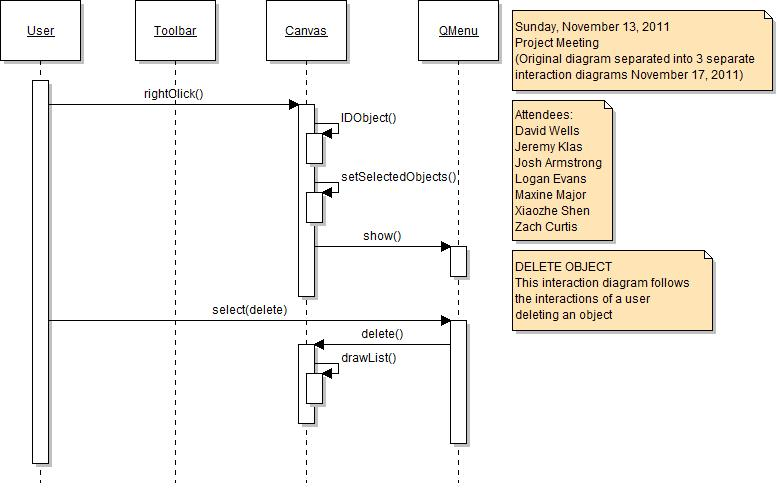
\includegraphics[width=6.0in]{IntDelObj.jpg}
\end{figure}

\clearpage


  

\subsubsection{Detailed Design for Feature: Delete a Connector}

\paragraph[\ Introduction/Purpose of this Feature]
{\ Introduction/Purpose of this Feature}
{\selectlanguage{english}\color{black}
The user deletes a connector from between two objects.
}

\paragraph[Input for this Feature]{Input for this Feature}
{\selectlanguage{english}\color{black}
The user right-clicks on an object to be deleted, and selects the delete option from the QMenu.
}

\paragraph{Output for this Feature}
{\selectlanguage{english}\color{black}
The Canvas deletes the connector.
}

\paragraph{Feature Process to Convert Input to Output}
{\selectlanguage{english}\color{black}
User right clicks on an connector on the Canvas. The Canvas verifies that an connector exists at the coordinates of the click, and sets the connector.  The Canvas prompts the QMenu to show itself.  The user selects the delete option from the QMenu.  The QMenu tells the Canvas to delete that connector. The Canvas deletes the connector and draws the updated list of connectors.
}

\paragraph{Design Constraints and Performance Requirements of this Feature}
{\selectlanguage{english}\color{black}
N/A
}
\bigskip
\bigskip

\begin{figure}[h]
\centering
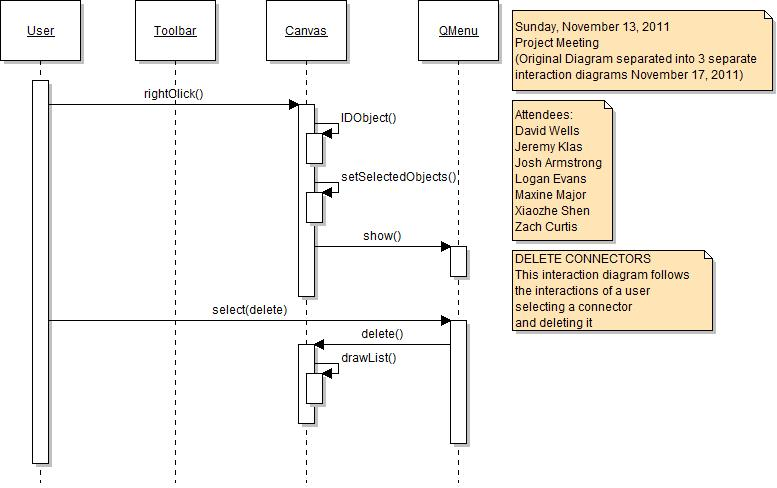
\includegraphics[width=6.0in]{IntDelConn.jpg}
\end{figure}

\clearpage

  


\subsubsection{Detailed Design for Feature: Save As }

\paragraph[\ Introduction/Purpose of this Feature]
{\ Introduction/Purpose of this Feature}
{\selectlanguage{english}\color{black}
The user wishes to save a UML diagram under a new file name.
}

\paragraph[Input for this Feature]{Input for this Feature}
{\selectlanguage{english}\color{black}
The user opens the File Menu and selects Save As.
}

\paragraph{Output for this Feature}
{\selectlanguage{english}\color{black}
pUML produces a QDialog box through which the user may type a new file name, and then saves the file.
}

\paragraph{Feature Process to Convert Input to Output}
{\selectlanguage{english}\color{black}
User clicks on the File menu option. User clicks on the Save As option. Main Menu creates a predefined QDialog and shows it to the user. The user types in the desired file name, and the QDialog submits this information to the Main Menu. Main Menu sends updated information about the file{\textquoteright}s saved status to the Canvas. Canvas acknowledges and returns xml.  Main Menu prints new xml information.
}

\paragraph{Design Constraints and Performance Requirements of this Feature}
{\selectlanguage{english}\color{black}
Directory browsing functionality within the QDialog may not be developed until a later release.
}
\bigskip
\bigskip

\begin{figure}[h]
\centering
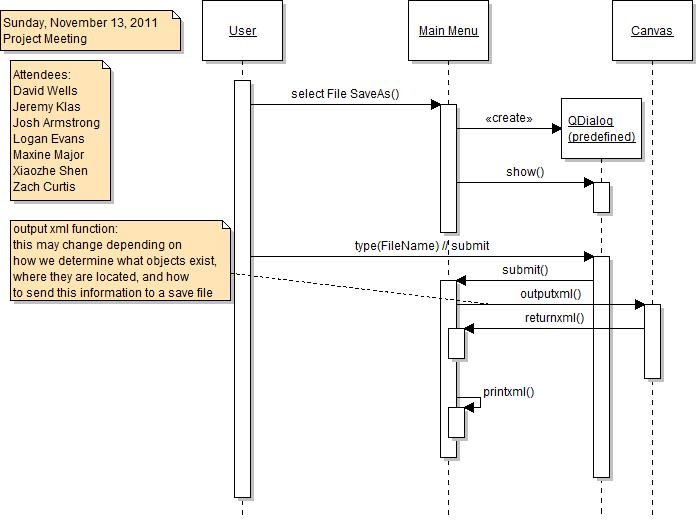
\includegraphics[width=6.0in]{IntSaveAs.jpg}
\end{figure}

\clearpage



\subsection{DATA DICTIONARY}

\begin{flushleft}
\tablehead{}
\begin{supertabular}{|m{0.9837598in}|m{0.9212598in}|m{1.8587599in}|m{1.2962599in}|m{1.1330599in}|}
\hline
\multicolumn{5}{|m{6.50806in}|}{\centering
\selectlanguage{english}\bfseries\color{black} Data Dictionary}\\\hline
\centering \selectlanguage{english}\bfseries\color{black} Name &
\centering \selectlanguage{english}\bfseries\color{black} Type/Range &
\centering \selectlanguage{english}\bfseries\color{black} Defined
by{\dots} &
\centering \selectlanguage{english}\bfseries\color{black} Referenced
by{\dots} &
\centering\arraybslash \selectlanguage{english}\bfseries\color{black}
Modified by{\dots}\\\hline
~ Main Window
 &
~ QMainWindow
 &
~ QWidget
 &
~ N/A
 &
~ User
\\\hline
~ Canvas
 &
~ QWidget
 &
~ QWidget
 &
~ Main Window
 &
~ User
\\\hline

\end{supertabular}
\end{flushleft}



\bigskip


\bigskip

\clearpage\setcounter{page}{1}\pagestyle{Convertvi}
\section[REQUIREMENTS
TRACEABILITY]{\selectlanguage{english}\rmfamily\bfseries\color{black}
REQUIREMENTS TRACEABILITY}


\bigskip

\begin{flushleft}
\tablehead{\hline
\multicolumn{1}{|m{0.9212598in}|}{\centering
\selectlanguage{english}\bfseries\color{black} Feature Name} &
\centering \selectlanguage{english}\bfseries\color{black} Req No. &
\centering \selectlanguage{english}\bfseries\color{black} Requirement
Description &
\centering \selectlanguage{english}\bfseries\color{black} Priority &
\centering \selectlanguage{english}\bfseries\color{black} SDD &
\multicolumn{2}{m{1.2872598in}|}{\centering
\selectlanguage{english}\bfseries\color{black} Alpha Release} &
\multicolumn{2}{m{1.3587599in}|}{\centering
\selectlanguage{english}\bfseries\color{black} Beta Release} &
\multicolumn{2}{m{1.3795599in}|}{\centering
\selectlanguage{english}\bfseries\color{black} Final Test}\\\hline
 &
 &
 &
 &
 &
\centering \selectlanguage{english}\bfseries\color{black} Test Case(s) &
\centering \selectlanguage{english}\bfseries\color{black} Test Res. &
\centering \selectlanguage{english}\bfseries\color{black} Test Case(s) &
\centering \selectlanguage{english}\bfseries\color{black} Test Res. &
\centering \selectlanguage{english}\bfseries\color{black} Test Case(s) &
\selectlanguage{english}\bfseries\color{black} Test
Res.\\\hhline{~~~~~------}}
\begin{supertabular}{m{0.9212598in}|m{0.42125985in}|m{1.9212599in}|m{0.39275986in}|m{0.7587598in}|m{0.6622598in}|m{0.5462598in}|m{0.6712598in}|m{0.6087598in}|m{0.6712598in}|m{0.6295598in}|}
\multicolumn{1}{|m{0.9212598in}|}{~Select Diagram Type
} &
\centering \selectlanguage{english}\color{black} 1.1 &
~Selects the appropriate diagram type
 &
~Mandatory
 &
~N/A
 &
~N/A
 &
~N/A
 &
~N/A
 &
~N/A
 &
~N/A
 &

~N/A
\\\hline
\multicolumn{1}{|m{0.9212598in}|}{~Save function
} &
\centering \selectlanguage{english}\color{black} 2.1 &
~Saves the Diagram to file
 &
~Mandatory
 &
~N/A
 &
~N/A
 &
~N/A
 &
~N/A
 &
~N/A
 &
~N/A
 &
~N/A
 
\\\hline
\multicolumn{1}{|m{0.9212598in}|}{~Draw function
} &
\centering \selectlanguage{english}\color{black} 2.1 &
~Draws current objects
 &
~Mandatory
 &
~N/A
 &
~N/A
 &
~N/A
 &
~N/A
 &
~N/A
 &
~N/A
 &
~N/A

\\\hline
\multicolumn{1}{|m{0.9212598in}|}{~Open File
} &
\centering \selectlanguage{english}\color{black} 2.1 &
~Opens previously saved file
 &
~Mandatory
 &
~N/A
 &
~N/A
 &
~N/A
 &
~N/A
 &
~N/A
 &
~N/A
 &
~N/A

\\\hline
\multicolumn{1}{|m{0.9212598in}|}{~New File
} &
\centering \selectlanguage{english}\color{black} 2.1 &
~Creates New File
 &
~Mandatory
 &
~N/A
 &
~N/A
 &
~N/A
 &
~N/A
 &
~N/A
 &
~N/A
 &
~N/A

\\\hline

\multicolumn{1}{|m{0.9212598in}|}{~SSRS and SSDD
} &
\centering \selectlanguage{english}\color{black} 2.1 &
~Too much work.
 &
~Mandatory
 &
~N/A
 &
~N/A
 &
~N/A
 &
~N/A
 &
~N/A
 &
~N/A



\\\hline
\end{supertabular}
\end{flushleft}
{\selectlanguage{english}\color{black}
Priorities are: \textbf{M}andatory, \textbf{L}ow, \textbf{H}igh}

{\selectlanguage{english}\color{black}
SDD link is version and page number or function name.}

{\selectlanguage{english}\color{black}
Test cases and results are file names and \textbf{P}ass/\textbf{F}ail or
\% passing.}

\clearpage\setcounter{page}{1}\pagestyle{Convertviii}

\end{document}